\documentclass[10pt,aspectratio=169]{beamer}
\usepackage{tikz}
\usepackage[utf8]{inputenc}
\usepackage[english]{babel}
\usepackage{verbatim}
\usepackage{listings}
\usetikzlibrary{positioning}
\usetikzlibrary{arrows}

\lstset{
  language=C++,                 % the language of the code
  backgroundcolor=\color{white},   % choose the background color; you must add \usepackage{color} or \usepackage{xcolor}
  basicstyle=\ttfamily\footnotesize,        % the size of the fonts that are used for the code
  columns=fullflexible,
  breakatwhitespace=false,         % sets if automatic breaks should only happen at whitespace
  breaklines=true,                 % sets automatic line breaking
  keywordstyle=\color{blue!80!black},       % keyword style
  captionpos=b,                    % sets the caption-position to bottom
  commentstyle=\color{green!50!black},       % comment style
  deletekeywords={},            % if you want to delete keywords from the given language
  escapeinside={\%*}{*)},          % if you want to add LaTeX within your code
  extendedchars=true,              % lets you use non-ASCII characters; for 8-bits encodings only, does not work with UTF-8
  frame=no,                    % adds a frame around the code
  keepspaces=true,                 % keeps spaces in text, useful for keeping indentation of code (possibly needs columns=flexible)
  morekeywords={using, static_assert, uint8_t, uint16_t, uint32_t, size_t},            % if you want to add more keywords to the set
  numbers=none,                    % where to put the line-numbers; possible values are (none, left, right)
  numbersep=7pt,                   % how far the line-numbers are from the code
  numberstyle=\tiny\color{black}, % the style that is used for the line-numbers
  rulecolor=\color{black},         % if not set, the frame-color may be changed on line-breaks within not-black text (e.g. comments (green here))
  showspaces=false,                % show spaces everywhere adding particular underscores; it overrides 'showstringspaces'
  showstringspaces=false,          % underline spaces within strings only
  showtabs=false,                  % show tabs within strings adding particular underscores
  stepnumber=1,                    % the step between two line-numbers. If it's 1, each line will be numbered
  stringstyle=\color{red},     % string literal style
  tabsize=2,                       % sets default tabsize to 2 spaces
  title=\lstname                   % show the filename of files included with \lstinputlisting; also try caption instead of title
}

%\makeatletter
%\define@key{beamerframe}{t}[true]{% top
%\beamer@frametopskip=.2cm plus .5\paperheight\relax%
%\beamer@framebottomskip=0pt plus 1fill\relax%
%\beamer@frametopskipautobreak=\beamer@frametopskip\relax%
%\beamer@framebottomskipautobreak=\beamer@framebottomskip\relax%
%\def\beamer@initfirstlineunskip{}%
%}
%\makeatother   

%__________________________________________________________

% Possible themes

%\usetheme{AnnArbor}       % Bad color
%\usetheme{Antibes}       % Not good
%\usetheme{Bergen}        % Wastes space
%\usetheme{Berkeley}      % Very good
%\usetheme{Berlin}        % Very good
%\usetheme{Boadilla}      % Good
%\usetheme{CambridgeUS}   % Very good but no section list
%\usetheme{Copenhagen}    %  Limpo
%\usetheme{Dresden}       %  Vale a pena tambem
%\usetheme{Frankfurt}     % limpo, com lista mas sem pagina
%\usetheme{Goettingen}    % Lista de secoes na lateral esquerda
%\usetheme{Hannover}      %  Lista de secoes na lateral direita sem pagina
%\usetheme{Ilmenau}       % Com secao e sub
%\usetheme{JuanLesPins}   % Mais ou menos
%\usetheme{Luebeck}       % Limpo e bem organizado
\usetheme{Madrid}        % So titulo e com pagina
%\usetheme{Malmoe}        % Nao tem caixa para o titulo
%\usetheme{Marburg}       % Bem organizado, sem caixa pra titulo e com lista na direita
%\usetheme{Montpellier}   % Nao gosto do design
%\usetheme{PaloAlto}      % Boa escolha
%\usetheme{Pittsburgh}    % Fraco
%\usetheme{Rochester}     % So caixa pro titulo
%\usetheme{Singapore}     % Fraco
%\usetheme{Szeged}        % Legal
%\usetheme{Warsaw}        % Bom
%\usetheme{boxes}         % Fraco
%\usetheme{default}       % Fraco
%__________________________________________________________

% Possible color themes

%\usecolortheme{albatross}
%\usecolortheme{beaver}         % Acho que é esse.
%\usecolortheme{beetle}        % Bom mas escuro
%\usecolortheme{crane}         % muito boa    
%\usecolortheme{default}        
%\usecolortheme{dolphin}      
%\usecolortheme{dove}          % legal
%\usecolortheme{fly}    
%\usecolortheme{lily}       
\usecolortheme{orchid}       
%\usecolortheme{seagull}       % excelente mas cinza
%\usecolortheme{seahorse}     
%\usecolortheme{sidebartab}    
%\usecolortheme{whale}       
%\usecolortheme{wolverine}       

\colorlet{memC}{brown!70!black}
\colorlet{eleC}{orange!70!black}

\colorlet{alertc}{red!80!black}

\colorlet{arraycontc}{green!70!black}
\colorlet{nodecontc}{blue!70!black}
\colorlet{bothcontc}{orange!70!black}

\tikzstyle{mbu}=[draw,node distance=0cm, fill=memC,shape=rectangle,minimum height=0.5cm  ,minimum width=0.5cm  ,inner sep=1ex]
\tikzstyle{mbd}=[draw,node distance=0cm, fill=memC,shape=rectangle,minimum height=0.5cm  ,minimum width=1.0cm  ,inner sep=1ex]
\tikzstyle{mbq}=[draw,node distance=0cm, fill=memC,shape=rectangle,minimum height=0.5cm  ,minimum width=2.0cm  ,inner sep=1ex]
\tikzstyle{mbo}=[draw,node distance=0cm, fill=memC,shape=rectangle,minimum height=0.5cm  ,minimum width=4.0cm  ,inner sep=1ex]

\tikzstyle{ebu}=[draw,node distance=0cm, fill=eleC,shape=rectangle,minimum height=0.5cm  ,minimum width=0.5cm  ,inner sep=1ex]
\tikzstyle{ebd}=[draw,node distance=0cm, fill=eleC,shape=rectangle,minimum height=0.5cm  ,minimum width=1.0cm  ,inner sep=1ex]
\tikzstyle{ebq}=[draw,node distance=0cm, fill=eleC,shape=rectangle,minimum height=0.5cm  ,minimum width=2.0cm  ,inner sep=1ex]
\tikzstyle{ebo}=[draw,node distance=0cm, fill=eleC,shape=rectangle,minimum height=0.5cm  ,minimum width=4.0cm  ,inner sep=1ex]

\tikzstyle{lbu}=[node distance=0cm, shape=rectangle,minimum height=0.5cm, minimum width=0.5cm, inner sep=1ex]
\tikzstyle{lbd}=[node distance=0cm, shape=rectangle,minimum height=0.5cm, minimum width=1.0cm, inner sep=1ex]
\tikzstyle{lbq}=[node distance=0cm, shape=rectangle,minimum height=0.5cm, minimum width=2.0cm, inner sep=1ex]
\tikzstyle{lbo}=[node distance=0cm, shape=rectangle,minimum height=0.5cm, minimum width=4.0cm, inner sep=1ex]

\tikzstyle{marrow}=[very thick, densely dotted,>=stealth,->, color=black]
\tikzstyle{earrow}=[very thick, >=stealth,->, color=black]
\tikzstyle{rearrow}=[very thick, >=stealth,<-, color=black]

\def\mbu{\node[style=mbu]}
\def\mbd{\node[style=mbd]}
\def\mbq{\node[style=mbq]}
\def\mbo{\node[style=mbo]}
\def\ebu{\node[style=ebu]}
\def\ebd{\node[style=ebd]}
\def\ebq{\node[style=ebq]}
\def\ebo{\node[style=ebo]}

\def\lbu{\node[style=lbu]}
\def\lbd{\node[style=lbd]}
\def\lbq{\node[style=lbq]}
\def\lbo{\node[style=lbo]}

\def\marrow{\draw[style=marrow]}
\def\earrow{\draw[style=earrow]}
\def\rearrow{\draw[style=rearrow]}

%__________________________________________________________
% Apenas para o tema madrid

%\defbeamertemplate*{footline}{my infolines theme}
%{
%  \leavevmode%
%    \hbox{%
%      \begin{beamercolorbox}[wd=.333333\paperwidth,ht=2.25ex,dp=1ex,center]{author in head/foot}%
%        \usebeamerfont{author in head/foot}\insertshortauthor~~\insertshortinstitute
%        \end{beamercolorbox}%
%        \begin{beamercolorbox}[wd=.333333\paperwidth,ht=2.25ex,dp=1ex,center]{title in head/foot}%
%        \usebeamerfont{title in head/foot}\insertshorttitle
%        \end{beamercolorbox}%
%        \begin{beamercolorbox}[wd=.333333\paperwidth,ht=2.25ex,dp=1ex,right]{date in head/foot}%
%        \usebeamerfont{date in head/foot}\insertshortdate{}\hspace*{2em}
%      \insertframenumber{} / \inserttotalframenumber\hspace*{2ex}
%      \end{beamercolorbox}}%
%        \vskip0pt%
%}
%__________________________________________________________

\mode<presentation>
{
  %\setbeamercovered{transparent}
   %\setbeamertemplate{footline}[frame number]
  % or whatever (possibly just delete it)
}

\title[Node allocation in STL containers] {Node allocation in STL containers}

\subtitle[Improving the memory menagement] {Improving the memory menagement}

\author[Marcelo Zimbres] {Marcelo Zimbres}

\institute[Presentation to WG21-SG14]
{
}

\date[Magstadt - Germany] {}

\subject{Node allocation 3}

% If you have a file called "university-logo-filename.xxx", where xxx
% is a graphic format that can be processed by latex or pdflatex,
% resp., then you can add a logo as follows:

%\pgfdeclareimage[height=1.2cm]{Wavelet}{fig/skymapJ8j2N127.pdf}
%\logo{\pgfuseimage{Wavelet}}

% Delete this, if you do not want the table of contents to pop up at
% the beginning of each subsection:
%\AtBeginSubsection[]
%{
%  \begin{frame}<beamer>{Outline}
%    %\tableofcontents[currentsection,currentsubsection]
%    \tableofcontents
%  \end{frame}
%}

% If you wish to uncover everything in a step-wise fashion, uncomment
% the following command: 

%\beamerdefaultoverlayspecification{<+->}

\begin{document}

%____________________________________________________________
\begin{frame}
  \titlepage
\end{frame}

%____________________________________________________________
%\begin{frame}{Outline}
%  \tableofcontents[pausesections]
%  % You might wish to add the option [pausesections]
%\end{frame}

%____________________________________________________________
%\begin{frame}<beamer>{Outline}
%   \tableofcontents[currentsection,currentsubsection]
%\end{frame}


% Since this a solution template for a generic talk, very little can
% be said about how it should be structured. However, the talk length
% of between 15min and 45min and the theme suggest that you stick to
% the following rules:  

% - Exactly two or three sections (other than the summary).
% - At *most* three subsections per section.
% - Talk about 30s to 2min per frame. So there should be between about
%   15 and 30 frames, all told.

%____________________________________________________________
\begin{frame}{Goals - Target audience}{}
\begin{columns}
\begin{column}{0.50\textwidth}
\begin{block} {Goals}
\begin{itemize}
    \item Provide building blocks for memory allocation.
    \item Profit from static type information.
    \item Reduce pointer overhead in nodes.
    \item Alternative to pointer chasing on traversal.
    \item Allow fine tunning and reduce complexity.
    \item Reduce centralization.
\end{itemize}
\end{block}

\end{column}

\begin{column}{0.35\textwidth}
\begin{block} {Target audience}
\begin{itemize}
    \item Embedded developers.
    \item Resource constrained systems.
    \item High performace.
    \item 24/7 availability.
\end{itemize}
\end{block}
\end{column}
\end{columns}
\end{frame}

%____________________________________________________________
\begin{frame}{Outline}
   %\tableofcontents[currentsection,currentsubsection]
   \tableofcontents
\end{frame}

\section{STL and memory management}

\subsection{Dynamic memory allocations in \texttt{C++}}

%____________________________________________________________
\begin{frame}[fragile]{Dynamic memory allocation in \texttt{C++}}
{Note: I will use {\it Heap} to refer free storage memory.}
\begin{columns}
\begin{column}[t]{0.45\textwidth}
\begin{block}{User level}
\begin{itemize}
\item Stack: Restricted lifetime, ``small''.
\item Heap: No restriction on lifetime and size.
\end{itemize}
\end{block}
%\vspace{0.5cm}
\begin{lstlisting}
int i; // Automatic allocation in the stack.

// C style heap allocation. No initialization.
int* p = malloc(sizeof *p);
free(p);

// C++ style heap allocation. Initializes.
auto* p = new int;
delete p;
\end{lstlisting}
\end{column}

\begin{column}[t]{0.45\textwidth}
\begin{block}{In STL containers}
\begin{itemize}
\item Stack and heap are abstracted away.
\item Memory is requested from allocators.
\end{itemize}
\end{block}
%\vspace{0.5cm}
\begin{lstlisting}
std::allocator<T> alloc; // Can have state.

// Requests enough space for one T.
auto* p = alloc.allocate(1);

alloc.construct(p, T()); // Calls ctor
alloc.destroy(p); // Calls dtor

// Return memory to the allocator.
alloc.deallocate(p, 1);

// See also std::allocator_traits.
\end{lstlisting}
\end{column}
\end{columns}
\end{frame}

%____________________________________________________________
\begin{frame}[fragile]
{Definitions (in the context of STL containers)}
\begin{columns}
\begin{column}{0.45\textwidth}

\begin{block} {Node allocation}
I will use {\bf \color{alertc} node allocation} to refer to
allocations that have always the same size.
\end{block}
\vspace{0.5cm}
\begin{lstlisting}
// e.g. allocations inside std::list
auto* p1 = alloc.allocate(1);
auto* p2 = alloc.allocate(1);
auto* p3 = alloc.allocate(1);
auto* p4 = alloc.allocate(1);
\end{lstlisting}

\end{column}

\begin{column}{0.45\textwidth}
\begin{block} {Array allocation}
For allocations with varying sizes I will use the term {\bf \color{alertc} array allocation}.
\end{block}
\vspace{0.5cm}
\begin{lstlisting}
// e.g. allocations inside std::vector
auto* p1 = alloc.allocate(2);
auto* p2 = alloc.allocate(4);
auto* p3 = alloc.allocate(8);
auto* p4 = alloc.allocate(16);
\end{lstlisting}
\end{column}
\end{columns}
\end{frame}

\subsection{Allocation patterns}

\begin{frame}{Containers and their allocation patterns}
\begin{columns}
\begin{column}[c]{0.45\textwidth}

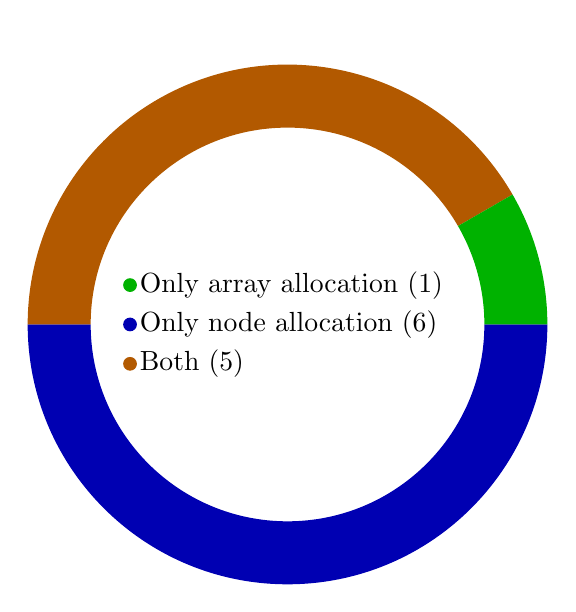
\begin{tikzpicture}[scale=1.0]
\fill[nodecontc]  (180:2.5cm) -- (180: 3.3cm) arc (180:360:3.3cm) -- (360:2.5cm) arc (360:180:2.5cm);
\fill[bothcontc]   (30:2.5cm) -- (30:3.3cm) arc (30:180:3.3cm)  -- (180:2.5cm) arc (180:30:2.5cm);
\fill[arraycontc] (0:2.5cm) -- (0:3.3cm) arc (0:30:3.3cm) -- (30:2.5cm) arc (30:0:2.5cm);

\filldraw[arraycontc] (-2cm,0.5cm) circle (0.08cm) node[right] {\color{black}Only array allocation (1)};
\filldraw[nodecontc] (-2cm,0.0cm) circle (0.08cm) node[right] {\color{black}Only node allocation (6)};
\filldraw[bothcontc] (-2cm,-0.5cm) circle (0.08cm) node[right] {\color{black}Both (5)};
\end{tikzpicture}
\end{column}

\begin{column}[c]{0.45\textwidth}
\begin{block} {STL containers (12)}
\begin{itemize}
\item \texttt{\color{arraycontc} std::vector}
\item \texttt{\color{nodecontc} std::list}
\item \texttt{\color{nodecontc} std::forward\_list}
\item \texttt{\color{nodecontc} std::set}
\item \texttt{\color{nodecontc} std::multiset}
\item \texttt{\color{nodecontc} std::map}
\item \texttt{\color{nodecontc} std::multimap}
\item \texttt{\color{bothcontc} std::deque}
\item \texttt{\color{bothcontc} std::unordered\_set}
\item \texttt{\color{bothcontc} std::unordered\_multiset}
\item \texttt{\color{bothcontc} std::unordered\_map}
\item \texttt{\color{bothcontc} std::unordered\_multimap}
\end{itemize}
\end{block}
\end{column}

\end{columns}
\end{frame}

%___________________________________________________________
\begin{frame}{Node allocation in the STL matters}

\begin{columns}
\begin{column}[c]{0.45\textwidth}
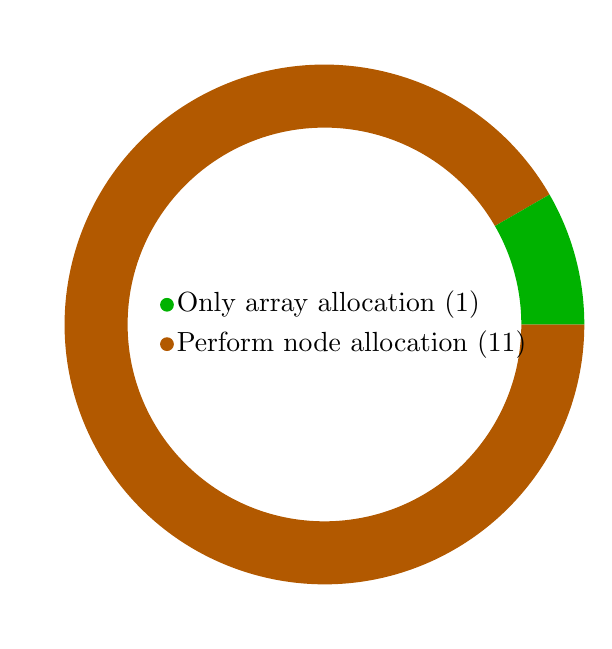
\begin{tikzpicture}[scale=1.0]
\fill[bothcontc]  (30:2.5cm) -- (30:3.3cm) arc (30:360:3.3cm) -- (360:2.5cm) arc (360:30:2.5cm);
\fill[arraycontc] (0:2.5cm) -- (0:3.3cm) arc (0:30:3.3cm) -- (30:2.5cm) arc (30:0:2.5cm);

\filldraw[arraycontc] (-2cm,0.25cm) circle (0.08cm) node[right] {\color{black} Only array allocation (1)};
\filldraw[bothcontc] (-2cm,-0.25cm) circle (0.08cm) node[right] {\color{black} Perform node allocation (11)};
\end{tikzpicture}
\end{column}

\begin{column}[c]{0.45\textwidth}
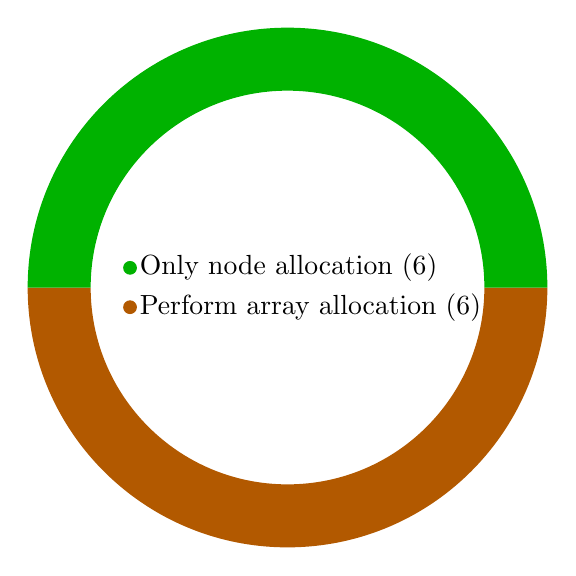
\begin{tikzpicture}[scale=1.0]
\fill[bothcontc]  (180:2.5cm) -- (180:3.3cm) arc (180:360:3.3cm) -- (360:2.5cm) arc (360:180:2.5cm);
\fill[arraycontc] (0:2.5cm) -- (0:3.3cm) arc (0:180:3.3cm) -- (180:2.5cm) arc (180:0:2.5cm);

\filldraw[arraycontc] (-2cm,0.25cm) circle (0.08cm) node[right] {\color{black} Only node allocation (6)};
\filldraw[bothcontc] (-2cm,-0.25cm) circle (0.08cm) node[right] {\color{black} Perform array allocation (6)};
\end{tikzpicture}
\end{column}
\end{columns}
\end{frame}

%____________________________________________________________
\begin{frame}[fragile]
{Why these information matters}
{A closer look at allocators}
\begin{columns}
\begin{column}{0.35\textwidth}

%\begin{block} {\texttt{allocate(n)}}
%\end{block}
\begin{lstlisting}
// Allocate signature.
pointer allocate(size_type n, ...);

void deallocate( pointer p
               , size_type n);
\end{lstlisting}

\end{column}

\begin{column}{0.55\textwidth}
\begin{block} {Allocators and size management}
\begin{itemize}
\item Allocation size is a runtime variable.
\item Node allocation is known at compile time.
\item Blesses array allocation. Unaware of node allocation.
\item No simple implementation. Has to handle any sizes.
\item Leads to overly complex strategies.
\item Leads to overheads like bookkeeping information.
\item Encourages centralization.
\end{itemize}

\end{block}

\end{column}
\end{columns}
\end{frame}
%____________________________________________________________
\begin{frame}[t]{Node allocation illustration}
{How it is implemented in practice: pooling}
\begin{block} {Procedure}
\begin{enumerate}
\item<alert@1> Get a continuos block of memory with enough space for $n$ nodes.
\item<alert@2> Divide in blocks, link them as a stack and repeat if ever run out of memory.
\item<alert@6> After some allocations and deallocations.
\end{enumerate}
\end{block}

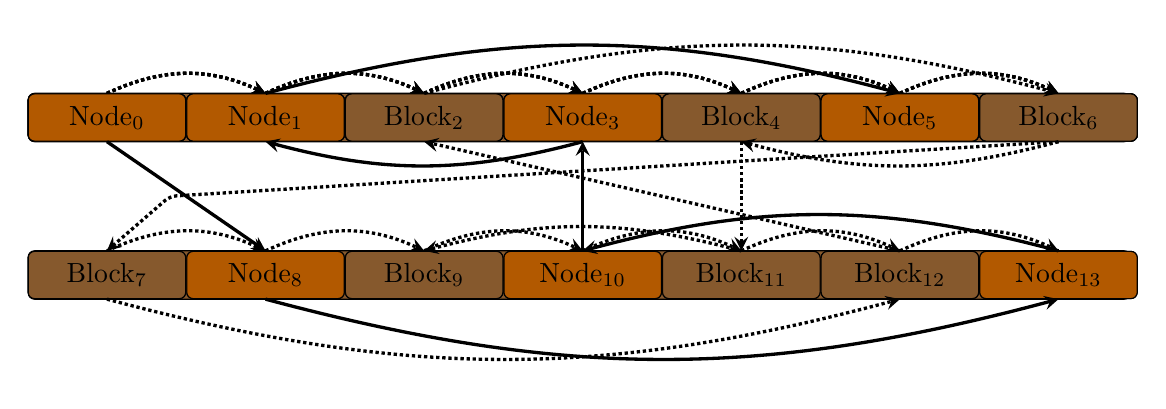
\begin{tikzpicture}[scale=1.0, rounded corners=0.8mm]

   \uncover<1> {
      \node[draw, node distance=0cm, fill=memC, shape=rectangle,minimum height=0.5cm  ,minimum width=14.0cm  ,inner sep=1ex]
      (block) at (1cm, 4cm) {Block with enough space for $n$ nodes};
   }

   \uncover<2> {
      \mbq (node0)  at (-5.0,4.0) {Block$_0$};
      \mbq (node1)  [right=of node0] {Block$_1$};
      \mbq (node2)  [right=of node1] {Block$_2$};
      \mbq (node3)  [right=of node2] {Block$_3$};
      \mbq (node4)  [right=of node3] {Block$_4$};
      \mbq (node5)  [right=of node4] {Block$_5$};
      \mbq (node6)  [right=of node5] {Block$_6$};
   }

   \uncover<3> {
      \mbq (node0)  at (-5.0,4.0) {Block$_0$};
      \mbq (node1)  [right=of node0] {Block$_1$};
      \mbq (node2)  [right=of node1] {Block$_2$};
      \mbq (node3)  [right=of node2] {Block$_3$};
      \mbq (node4)  [right=of node3] {Block$_4$};
      \mbq (node5)  [right=of node4] {Block$_5$};
      \mbq (node6)  [right=of node5] {Block$_6$};

      \marrow (node0.north) to [bend right=-25] (node1.north);
      \marrow (node1.north) to [bend right=-25] (node2.north);
      \marrow (node2.north) to [bend right=-25] (node3.north);
      \marrow (node3.north) to [bend right=-25] (node4.north);
      \marrow (node4.north) to [bend right=-25] (node5.north);
      \marrow (node5.north) to [bend right=-25] (node6.north);
   }

   \uncover<4> {
      \mbq (node0)  at (-5.0,4.0) {Block$_0$};
      \mbq (node1)  [right=of node0] {Block$_1$};
      \mbq (node2)  [right=of node1] {Block$_2$};
      \mbq (node3)  [right=of node2] {Block$_3$};
      \mbq (node4)  [right=of node3] {Block$_4$};
      \mbq (node5)  [right=of node4] {Block$_5$};
      \mbq (node6)  [right=of node5] {Block$_6$};

      \marrow (node0.north) to [bend right=-25] (node1.north);
      \marrow (node1.north) to [bend right=-25] (node2.north);
      \marrow (node2.north) to [bend right=-25] (node3.north);
      \marrow (node3.north) to [bend right=-25] (node4.north);
      \marrow (node4.north) to [bend right=-25] (node5.north);
      \marrow (node5.north) to [bend right=-25] (node6.north);

      \node[draw, node distance=0cm, fill=memC, shape=rectangle,minimum height=0.5cm  ,minimum width=14.0cm  ,inner sep=1ex]
      (block) at (1cm, 2cm) {Run out of memory, get another block. };
   }

   \uncover<5> {
      \mbq (node0)  at (-5.0,4.0) {Block$_0$};
      \mbq (node1)  [right=of node0] {Block$_1$};
      \mbq (node2)  [right=of node1] {Block$_2$};
      \mbq (node3)  [right=of node2] {Block$_3$};
      \mbq (node4)  [right=of node3] {Block$_4$};
      \mbq (node5)  [right=of node4] {Block$_5$};
      \mbq (node6)  [right=of node5] {Block$_6$};

      \mbq (node7)  at (-5.0,2.0)     {Block$_7$};
      \mbq (node8)  [right=of node7] {Block$_8$};
      \mbq (node9)  [right=of node8] {Block$_9$};
      \mbq (node10) [right=of node9] {Block$_{10}$};
      \mbq (node11) [right=of node10] {Block$_{11}$};
      \mbq (node12) [right=of node11] {Block$_{12}$};
      \mbq (node13) [right=of node12] {Block$_{13}$};

      \marrow (node0.north) to [bend right=-25] (node1.north);
      \marrow (node1.north) to [bend right=-25] (node2.north);
      \marrow (node2.north) to [bend right=-25] (node3.north);
      \marrow (node3.north) to [bend right=-25] (node4.north);
      \marrow (node4.north) to [bend right=-25] (node5.north);
      \marrow (node5.north) to [bend right=-25] (node6.north);

      \marrow (node6.south)  -- (-4.2, 3.0) -- (node7.north);
      \marrow (node7.north)  to [bend right=-25] (node8.north);
      \marrow (node8.north)  to [bend right=-25] (node9.north);
      \marrow (node9.north)  to [bend right=-25] (node10.north);
      \marrow (node10.north) to [bend right=-25] (node11.north);
      \marrow (node11.north) to [bend right=-25] (node12.north);
      \marrow (node12.north) to [bend right=-25] (node13.north);
   }

   \uncover<6-> {
      \ebq (node0)  at (-5.0,4.0) {Node$_0$};
      \ebq (node1)  [right=of node0] {Node$_1$};
      \mbq (node2)  [right=of node1] {Block$_2$};
      \ebq (node3)  [right=of node2] {Node$_3$};
      \mbq (node4)  [right=of node3] {Block$_4$};
      \ebq (node5)  [right=of node4] {Node$_5$};
      \mbq (node6)  [right=of node5] {Block$_6$};

      \mbq (node7)  at (-5.0,2.0)     {Block$_7$};
      \ebq (node8)  [right=of node7] {Node$_8$};
      \mbq (node9)  [right=of node8] {Block$_9$};
      \ebq (node10) [right=of node9] {Node$_{10}$};
      \mbq (node11) [right=of node10] {Block$_{11}$};
      \mbq (node12) [right=of node11] {Block$_{12}$};
      \ebq (node13) [right=of node12] {Node$_{13}$};
   }

   \uncover<6-> {
      \earrow (node0.south) -- (node8.north);
      \earrow (node1.north) to [bend right=-15] (node5.north);
      \earrow (node3.south) to [bend right=-15] (node1.south);
      \earrow (node8.south) to [bend right=15] (node13.south);
      \earrow (node10.north) -- (node3.south);
      \earrow (node13.north) to [bend right=15] (node10.north);
   }

   \uncover<6-> {
      \marrow (node2.north) to [bend right=-15] (node6.north);
      \marrow (node6.south) to [bend right=-15] (node4.south);
      \marrow (node4.south) -- (node11.north);
      \marrow (node11.north) to [bend right=15] (node9.north);
      \marrow (node7.south) to [bend right=15] (node12.south);
      \marrow (node12.north) -- (node2.south);
   }

\end{tikzpicture}

\end{frame}

%____________________________________________________________
\begin{frame}[fragile]
{Simplicity matters}
{How node allocation is implemented}

\begin{center}
\begin{lstlisting}
                         pointer allocate_node()
                         {
                           pointer q = avail; // The next free node
                           if (avail)
                             avail = avail->next;
                         
                           return q;
                         }
                         
                         void deallocate_node(pointer p)
                         {
                           p->next = avail;
                           avail = p;
                         }

\end{lstlisting}
\end{center}
\end{frame}

%____________________________________________________________
\begin{frame}{Outline}
   \tableofcontents[currentsection,currentsubsection]
\end{frame}

\subsection{Typical allocation goals and strategies}

%____________________________________________________________
\begin{frame}{Typical allocation goals and strategies}
{\texttt{malloc}, \texttt{jemalloc}, \texttt{tcmalloc},
\texttt{nedmalloc}, \texttt{hoard}, etc.}
\begin{columns}
\begin{column}{0.47\textwidth}
\begin{block} {Typical goals and strategies}
\begin{itemize}
\item Different strategy for small and big sizes.
\item Small sizes: Many pre-allocated blocks.
\item Large sizes: Best fit, rounding on memory pages.
\item Avoid fragmentation. Improve locality.
\item Avoid serialization on cuncurrent calls.
\item Thread local buffers.
\item Bookkeeping information on blocks.
\item Rounding allocation sizes to fit pre-allocated buffers.
\end{itemize}
\end{block}
\end{column}

\begin{column}{0.47\textwidth}
\begin{block} {Centralization is bad}
If basic building blocks were available i.e. node allocation,
many of these problems could be properly handled e.g.
bookkeeping information, rounding, size searches
are unnecessary on node allocation. Compile time information would not
be thrown away.
\end{block}

\end{column}
\end{columns}
\end{frame}

\subsection{Node allocation as a building block}

%___________________________________________________________________
\begin{frame}[t]{Pools of blocks with different sizes}
\begin{block}{Why all this if the exact sizes are available
at compile time?}
\begin{itemize}
\item Many pre-allocated sizes. Possibly thread local.
\item Small sizes are rounded to one of these.
\item \texttt{std::malloc} has up to 170 of these lists.
\end{itemize}
\end{block}
\vspace{0.5cm}
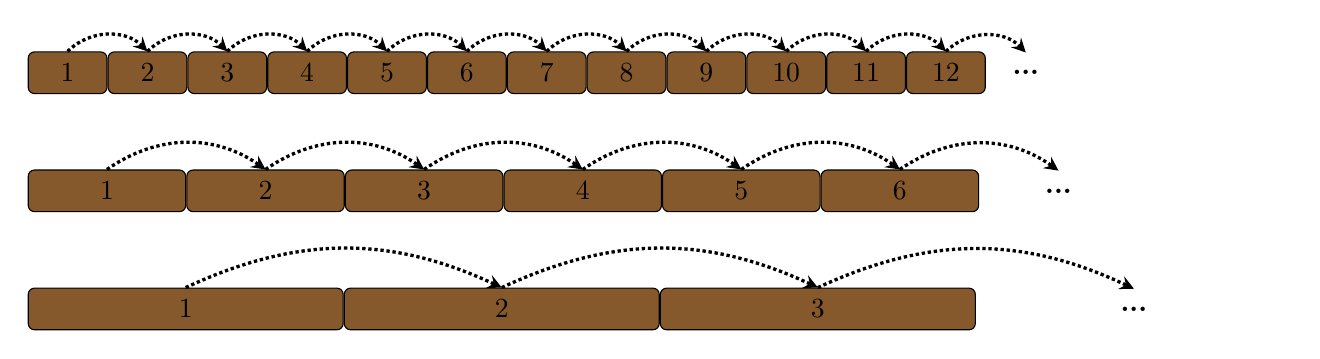
\begin{tikzpicture}[scale=1.0, rounded corners=0.8mm]
      % next
      \mbd (Unode0) at  (0.5,2.0)       {1};
      \mbd (Unode1)  [right=of Unode0]  {2};
      \mbd (Unode2)  [right=of Unode1]  {3};
      \mbd (Unode3)  [right=of Unode2]  {4};
      \mbd (Unode4)  [right=of Unode3]  {5};
      \mbd (Unode5)  [right=of Unode4]  {6};
      \mbd (Unode6)  [right=of Unode5]  {7};
      \mbd (Unode7)  [right=of Unode6]  {8};
      \mbd (Unode8)  [right=of Unode7]  {9};
      \mbd (Unode9)  [right=of Unode8]  {10};
      \mbd (Unode10) [right=of Unode9]  {11};
      \mbd (Unode11) [right=of Unode10] {12};
      \lbd (Unode12) [right=of Unode11] {\bf ...};

      \marrow (Unode0.north) to  [bend right=-45] (Unode1.north);
      \marrow (Unode1.north) to  [bend right=-45] (Unode2.north);
      \marrow (Unode2.north) to  [bend right=-45] (Unode3.north);
      \marrow (Unode3.north) to  [bend right=-45] (Unode4.north);
      \marrow (Unode4.north) to  [bend right=-45] (Unode5.north);
      \marrow (Unode5.north) to  [bend right=-45] (Unode6.north);
      \marrow (Unode6.north) to  [bend right=-45] (Unode7.north);
      \marrow (Unode7.north) to  [bend right=-45] (Unode8.north);
      \marrow (Unode8.north) to  [bend right=-45] (Unode9.north);
      \marrow (Unode9.north) to  [bend right=-45] (Unode10.north);
      \marrow (Unode10.north) to [bend right=-45] (Unode11.north);
      \marrow (Unode11.north) to [bend right=-45] (Unode12.north);
      % next
      \mbq (Qnode0) at  (1.0,0.5)      {1};
      \mbq (Qnode1)  [right=of Qnode0] {2};
      \mbq (Qnode2)  [right=of Qnode1] {3};
      \mbq (Qnode3)  [right=of Qnode2] {4};
      \mbq (Qnode4)  [right=of Qnode3] {5};
      \mbq (Qnode5)  [right=of Qnode4] {6};
      \lbq (Qnode6)  [right=of Qnode5] {\bf ...};

      \marrow (Qnode0.north) to  [bend right=-35] (Qnode1.north);
      \marrow (Qnode1.north) to  [bend right=-35] (Qnode2.north);
      \marrow (Qnode2.north) to  [bend right=-35] (Qnode3.north);
      \marrow (Qnode3.north) to  [bend right=-35] (Qnode4.north);
      \marrow (Qnode4.north) to  [bend right=-35] (Qnode5.north);
      \marrow (Qnode5.north) to  [bend right=-35] (Qnode6.north);
      % next
      \mbo (Onode0) at  (2.0,-1.0)     {1};
      \mbo (Onode1)  [right=of Onode0] {2};
      \mbo (Onode2)  [right=of Onode1] {3};
      \lbo (Onode3)  [right=of Onode2] {\bf ...};

      \marrow (Onode0.north) to [bend right=-25] (Onode1.north);
      \marrow (Onode1.north) to [bend right=-25] (Onode2.north);
      \marrow (Onode2.north) to [bend right=-25] (Onode3.north);

\end{tikzpicture}
\end{frame}

%_________________________________________________________________________

\begin{frame}[fragile]{Further thoughts}
\begin{itemize}
\item Many possible strategies. Which one should I use?
\item Has to handle different sizes.
\item No silver bullet. Every problem requires a different approach.
\item Users do not want to care about this unless there is need.
\item malloc: suitable for large memory blocks, overused, hundreds of
\item LOC, system calls, etc.
\item May use node allocation as a building block.
\end{itemize}

\end{frame}

%____________________________________________________________
\begin{frame}[fragile]
{}

\begin{columns}
\begin{column}{0.15\textwidth}
\end{column}
\begin{column}{0.70\textwidth}
\begin{center}
 \Large \bf 
  I've been arguing that node allocation is an important concept and deserves
  support in the STL. Now lets us see how to do it and what further benefits
  it will bring.
\end{center}
\end{column}
\begin{column}{0.15\textwidth}
\end{column}
\end{columns}
\end{frame}

\section{Supporting node-allocation in the STL}
\subsection{Proposal}

%____________________________________________________________
\begin{frame}{Outline}
   \tableofcontents[currentsection,currentsubsection]
\end{frame}

%____________________________________________________________
\begin{frame}{Should node allocation be standardized}{Proposal to the ISO \texttt{C++} Standards Committee}
\vspace{-3cm}
    \begin{center}
        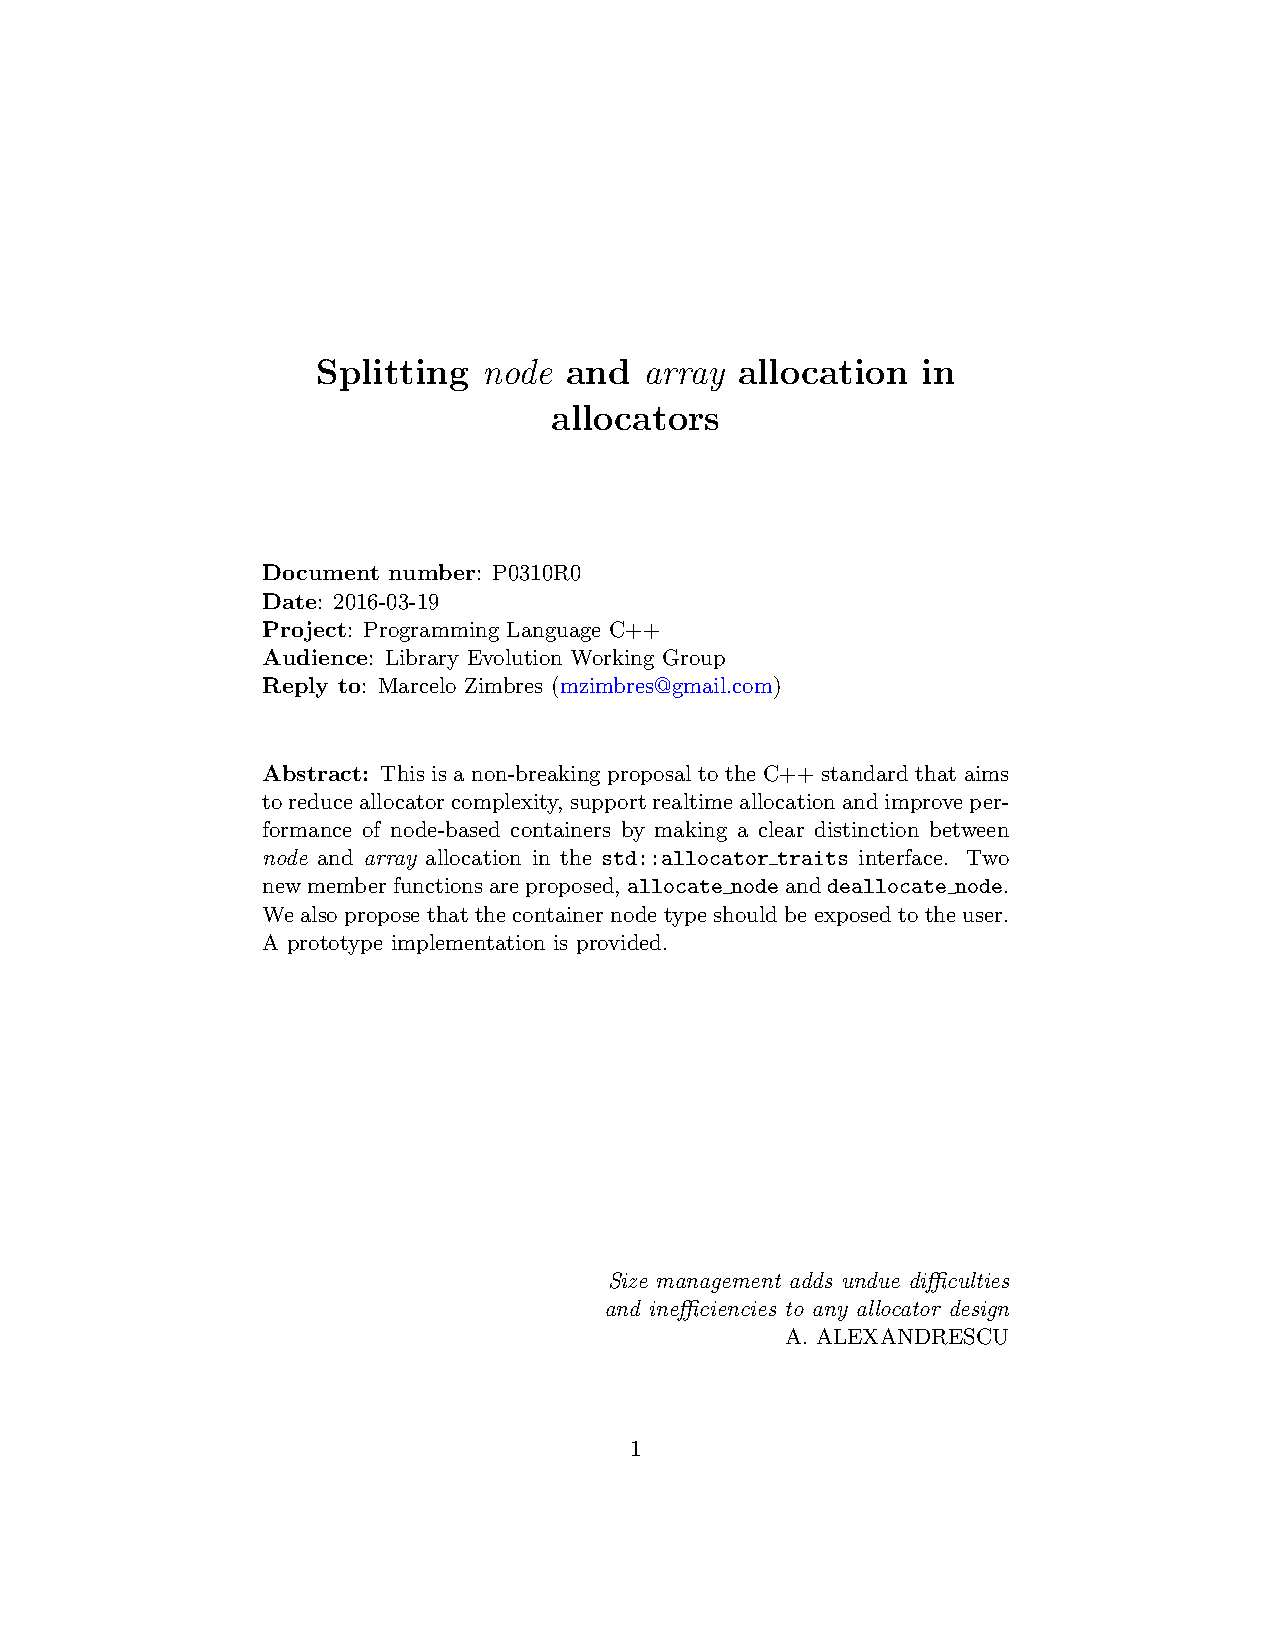
\includegraphics[scale=0.6]{fig/prop1.pdf} \\
    \end{center}
\end{frame}

%____________________________________________________________
\begin{frame}[fragile]{Node allocation support}

\begin{lstlisting}
template<class Alloc>
struct allocator_traits {
  // Equal to Alloc::node_allocation_only if present,
  // std::false_type otherwise. Array allocation with
  // allocate(n) is ruled out if it is std::true_type.
  using node_allocation_only = std::false_type
  // Calls a.allocate_node() if present otherwise calls
  // Alloc::allocate(1). Memory allocate with this function
  // must be deallocated with deallocate_node.
  pointer allocate_node(Alloc& a);
  // Calls a.deallocate_node(pointer) if present otherwise
  // calls Alloc::deallocate(p, 1). Can only be used with
  // memory allocated with allocate_node.
  void deallocate_node(Alloc& a, pointer p);
};
\end{lstlisting}

\end{frame}

%____________________________________________________________
\begin{frame}[fragile]{Exposing the node type}{Fancy pointers}

\begin{lstlisting}
// Cannot always hold for general A1 nd A2.
static_assert( std::is_same< std::list<T, A1>::node_type
                           , std::list<T, A2>::node_type>, "");
\end{lstlisting}

\end{frame}

%____________________________________________________________
\begin{frame}[fragile]{Exposing the node type}{Node type interface}

\begin{lstlisting}
template <class T, class Ptr>
struct node_type {
  using value_type = T;
  using pointer = // Usually taken from std::pointer_traits<Ptr>
  template<class U, class K>
  struct rebind { using other = node_type<U , K>; };
  // ... implementation details
\end{lstlisting}

\end{frame}

%____________________________________________________________
\begin{frame}[fragile]{Example}

\begin{lstlisting}
using alloc_t = rt::node_allocator<int>;
using node_type = typename std::list<int, alloc_t>::node_type;

// Buffer for 100 elements.
std::array<char, 100 * sizeof (node_type)> buffer = {{}};
alloc_t alloc(buffer);

std::list<int, alloc_t> l1(alloc);
// Inserts elements. Allocation and deallocation implemented
// with 6 lines of code.
l1 = {27, 1, 60};
...
\end{lstlisting}

\end{frame}

%____________________________________________________________
\begin{frame}{Bechmarks}
    \begin{columns}
        \begin{column}{0.5\textwidth}
            \texttt{std::unordered\_set}
            \begin{center}
                \includegraphics[scale=0.6]{fig/unordered_set_with_frag.pdf} \\
            \end{center}
        \end{column}

        \begin{column}{0.5\textwidth}
            \texttt{std::set}
            \begin{center}
                \includegraphics[scale=0.6]{fig/set_bench.pdf} \\
            \end{center}
        \end{column}
    \end{columns}
\end{frame}

\subsection{Traversal without pointer chasing}

%____________________________________________________________
\begin{frame}[fragile]{Linked list travesal illustration}
\begin{columns}
\begin{column}{0.6\textwidth}
\begin{block} {Can we avoid chasing pointers?}
\begin{enumerate}
\item<alert@1> Initial memory state. Available memory.
\item<alert@2> After insertion and removal we have chaos.
\item<alert@3> Traversal chasing pointers jumps to slow memory.
\item<alert@4> Alternative: Visit blocks sequentially. Ignore unused.
\end{enumerate}
\end{block}
\end{column}
\begin{column}{0.4\textwidth}

\end{column}
\end{columns}

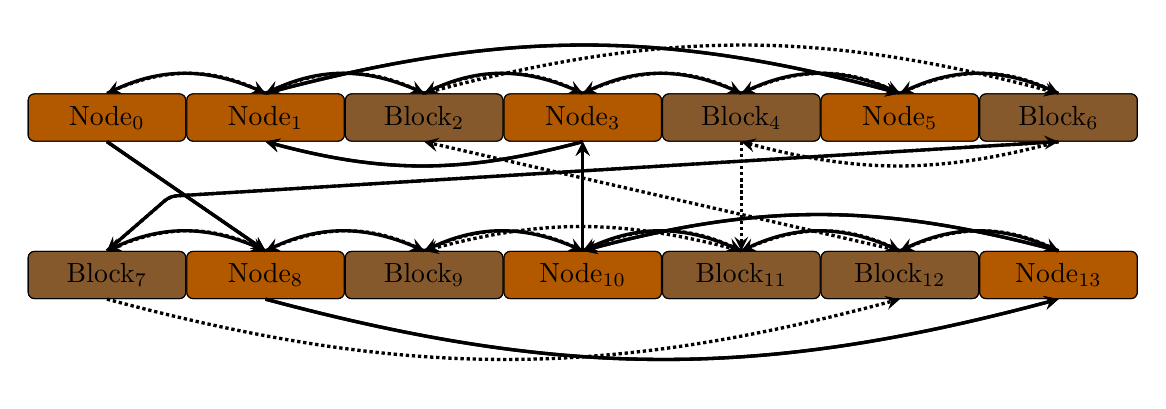
\begin{tikzpicture}[scale=1.0, rounded corners=0.8mm]

   \uncover<1> {
      \mbq (node0)  at (-5.0,4.0) {Block$_0$};
      \mbq (node1)  [right=of node0] {Block$_1$};
      \mbq (node2)  [right=of node1] {Block$_2$};
      \mbq (node3)  [right=of node2] {Block$_3$};
      \mbq (node4)  [right=of node3] {Block$_4$};
      \mbq (node5)  [right=of node4] {Block$_5$};
      \mbq (node6)  [right=of node5] {Block$_6$};

      \mbq (node7)  at (-5.0,2.0)     {Block$_7$};
      \mbq (node8)  [right=of node7] {Block$_8$};
      \mbq (node9)  [right=of node8] {Block$_9$};
      \mbq (node10) [right=of node9] {Block$_{10}$};
      \mbq (node11) [right=of node10] {Block$_{11}$};
      \mbq (node12) [right=of node11] {Block$_{12}$};
      \mbq (node13) [right=of node12] {Block$_{13}$};

      \marrow (node0.north) to [bend right=-25] (node1.north);
      \marrow (node1.north) to [bend right=-25] (node2.north);
      \marrow (node2.north) to [bend right=-25] (node3.north);
      \marrow (node3.north) to [bend right=-25] (node4.north);
      \marrow (node4.north) to [bend right=-25] (node5.north);
      \marrow (node5.north) to [bend right=-25] (node6.north);

      \marrow (node6.south)  -- (-4.2, 3.0) -- (node7.north);
      \marrow (node7.north)  to [bend right=-25] (node8.north);
      \marrow (node8.north)  to [bend right=-25] (node9.north);
      \marrow (node9.north)  to [bend right=-25] (node10.north);
      \marrow (node10.north) to [bend right=-25] (node11.north);
      \marrow (node11.north) to [bend right=-25] (node12.north);
      \marrow (node12.north) to [bend right=-25] (node13.north);
   }

   \uncover<2-> {
      \ebq (node0)  at (-5.0,4.0) {Node$_0$};
      \ebq (node1)  [right=of node0] {Node$_1$};
      \mbq (node2)  [right=of node1] {Block$_2$};
      \ebq (node3)  [right=of node2] {Node$_3$};
      \mbq (node4)  [right=of node3] {Block$_4$};
      \ebq (node5)  [right=of node4] {Node$_5$};
      \mbq (node6)  [right=of node5] {Block$_6$};

      \mbq (node7)  at (-5.0,2.0)     {Block$_7$};
      \ebq (node8)  [right=of node7] {Node$_8$};
      \mbq (node9)  [right=of node8] {Block$_9$};
      \ebq (node10) [right=of node9] {Node$_{10}$};
      \mbq (node11) [right=of node10] {Block$_{11}$};
      \mbq (node12) [right=of node11] {Block$_{12}$};
      \ebq (node13) [right=of node12] {Node$_{13}$};
   }

   \uncover<2> {
      \earrow (node0.south) -- (node8.north);
      \earrow (node1.north) to [bend right=-15] (node5.north);
      \earrow (node3.south) to [bend right=-15] (node1.south);
      \earrow (node8.south) to [bend right=15] (node13.south);
      \earrow (node10.north) -- (node3.south);
      \earrow (node13.north) to [bend right=15] (node10.north);
   }

   \uncover<2> {
      \marrow (node2.north) to [bend right=-15] (node6.north);
      \marrow (node6.south) to [bend right=-15] (node4.south);
      \marrow (node4.south) -- (node11.north);
      \marrow (node11.north) to [bend right=15] (node9.north);
      \marrow (node7.south) to [bend right=15] (node12.south);
      \marrow (node12.north) -- (node2.south);
   }

   \uncover<3> {
      \earrow (node0.south) -- (node8.north);
      \earrow (node1.north) to [bend right=-15] (node5.north);
      \earrow (node3.south) to [bend right=-15] (node1.south);
      \earrow (node8.south) to [bend right=15] (node13.south);
      \earrow (node10.north) -- (node3.south);
      \earrow (node13.north) to [bend right=15] (node10.north);
   }


   \uncover<4> {
      \rearrow (node0.north) to [bend right=-25] (node1.north);
      \rearrow (node1.north) to [bend right=-25] (node2.north);
      \rearrow (node2.north) to [bend right=-25] (node3.north);
      \rearrow (node3.north) to [bend right=-25] (node4.north);
      \rearrow (node4.north) to [bend right=-25] (node5.north);
      \rearrow (node5.north) to [bend right=-25] (node6.north);

      \rearrow (node6.south)  -- (-4.2, 3.0) -- (node7.north);
      \rearrow (node7.north)  to [bend right=-25] (node8.north);
      \rearrow (node8.north)  to [bend right=-25] (node9.north);
      \rearrow (node9.north)  to [bend right=-25] (node10.north);
      \rearrow (node10.north) to [bend right=-25] (node11.north);
      \rearrow (node11.north) to [bend right=-25] (node12.north);
      \rearrow (node12.north) to [bend right=-25] (node13.north);
   }

\end{tikzpicture}

\end{frame}

%____________________________________________________________
\begin{frame}{Why it is so important to avoid jumping around}{Cache Hierarchy - Speed}
    \begin{columns}
        \begin{column}{0.33\textwidth}

        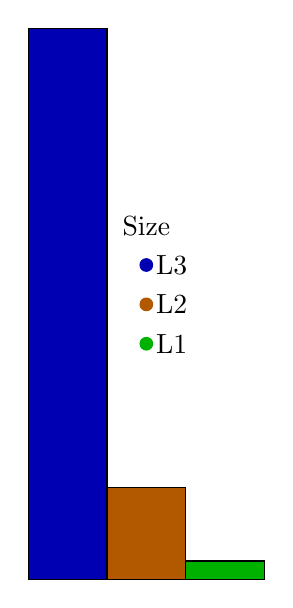
\begin{tikzpicture}[scale=1.0]
        \node[anchor=south, draw,node distance=0cm, fill=nodecontc,shape=rectangle,minimum height=7.0cm  ,minimum width=1.0cm]
        (node0) at (0cm,0cm) {};
        \node[anchor=south,draw,node distance=0cm, fill=bothcontc,shape=rectangle,minimum height=1.17cm  ,minimum width=1.0cm]
        (node1) at (1cm,0.0cm) {};
        \node[anchor=south,draw,node distance=0cm, fill=arraycontc,shape=rectangle,minimum height=0.15cm  ,minimum width=1.0cm]
        (node2) at (2cm,0cm) {};

        \node[] at (1cm,4.5cm) {\color{black} Size};
        \filldraw[nodecontc] (1cm,4.0cm) circle (0.08cm) node[right] {\color{black} L3};
        \filldraw[bothcontc] (1cm,3.5cm) circle (0.08cm) node[right] {\color{black}L2};
        \filldraw[arraycontc] (1cm,3.0cm) circle (0.08cm) node[right] {\color{black}L1};

        \end{tikzpicture}
        \end{column}

        \begin{column}{0.33\textwidth}

        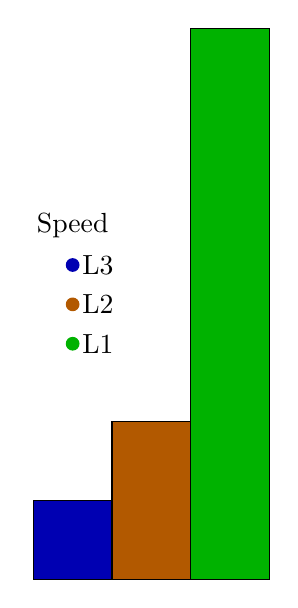
\begin{tikzpicture}[scale=1.0]
        \node[anchor=south, draw,node distance=0cm, fill=nodecontc,shape=rectangle,minimum height=1.00cm  ,minimum width=1.0cm]
        (node0) at (0cm,0cm) {};
        \node[anchor=south,draw,node distance=0cm, fill=bothcontc,shape=rectangle,minimum height=2.00cm  ,minimum width=1.0cm]
        (node1) at (1cm,0.0cm) {};
        \node[anchor=south,draw,node distance=0cm, fill=arraycontc,shape=rectangle,minimum height=7.00cm  ,minimum width=1.0cm]
        (node2) at (2cm,0cm) {};

        \node[] at (0cm,4.5cm) {\color{black} Speed};
        \filldraw[nodecontc] (0cm,4.0cm) circle (0.08cm) node[right] {\color{black} L3};
        \filldraw[bothcontc] (0cm,3.5cm) circle (0.08cm) node[right] {\color{black}L2};
        \filldraw[arraycontc] (0cm,3.0cm) circle (0.08cm) node[right] {\color{black}L1};

        \end{tikzpicture}
        \end{column}

        \begin{column}{0.3\textwidth}
            Intel Haswell Mobile 
            \begin{itemize}
                \item Register: Fastest
                \item L0: 6 KiB
                \item L1: 128 KiB - 700 GiB/s
                \item L2: 1 MiB - 200 GiB/s
                \item L3: 6 MiB - 100 GB/s
                \item L4: 128 MiB - 40 GB/s
                \item Main memory – GiB - 10 GB/s
            \end{itemize}
        \end{column}

    \end{columns}
\end{frame}

%____________________________________________________________
\begin{frame}[fragile]{Alternative to pointer chasing}
\begin{block} {Code example}
\begin{itemize}
\item User provides a function to mark the \texttt{value\_type}
as {\it in use}.
\item \texttt{allocate(1)} and \texttt{deallocate(1)} calls that 
function.
\item The node type must obviously be exposed.
\end{itemize}
\end{block}

\begin{lstlisting}
using node_type = std::list<int>::node_type;
// Allocator configured to allocator chuncks of 256
// elements at once.
using alloc_type = node_allocator<node_type, 256>;
std::list<int, node_allocator<>> l = {1, 2, 3, 4, 5};
auto alloc = l.get_allocator();
std::copy(std::begin(alloc), std::end(alloc),
 std::ostream_iterator<node_type>(std::cout, " "))
\end{lstlisting}

\end{frame}

\subsection{Reducing the pointer overhead in nodes}

%____________________________________________________________
\begin{frame}[fragile]{Reducing the pointer overhead in nodes}
\begin{quotation}
\noindent
It is absolutely idiotic to have 64-bit pointers when I compile a program that
uses less than 4 gigabytes of RAM. When such pointer values appear inside a
struct, they not only waste half the memory, they effectively throw away half
of the cache.
\end{quotation}
(Donald Knuth)
\end{frame}

\begin{frame}[fragile]{Nodes and pointers}
\begin{columns}
\begin{column}{0.5\textwidth}

\begin{lstlisting}
          struct node {
            node* next;
            int info;
          };
\end{lstlisting}
\end{column}
\begin{column}{0.5\textwidth}
\begin{block}{Thoughts}
\begin{itemize}
\item On a 64 bits system the size of the node on the left is 16 bytes.
\item 4 bytes by are wasted on padding.
\item Using 32 bits pointers may not be an option.
\item Even if it were, for only hundres of elements
8 or 16 bits are enough to address the elements.
\end{itemize}
\end{block}

\end{column}
\end{columns}

\end{frame}

%____________________________________________________________
\begin{frame}[fragile]{What if I could address elements with integers}
\begin{columns}
\begin{column}{0.5\textwidth}
%\begin{enumerate}
%\item<alert@1> $N \le 256$ with $T \in [0, 256]$
%\item<alert@2> $N \le 2^{16}$ with $T \in [0, 2^{16}]$
%\item<alert@3> $N \le 2^{32}$ with $T \in [0, 2^{32}]$
%\item<alert@4> $N \le 2^{64}$ with $T \in [0, 2^{64}]$
%\end{enumerate}

%Node sizes of a \texttt{std::forwar\_list<T>}.

%\begin{tikzpicture}[scale=1.0, rounded corners=0.8mm]
%
%   \uncover<1-> {
%      \mbu (nextu) at (0.25, 6) {N};
%      \ebu (valueu) [right=of nextu] {V};
%   }
%
%   \uncover<2-> {
%      \mbd (nextd) at (0.5,4) {Next};
%      \ebd (valued) [right=of nextd] {Value};
%   }
%
%   \uncover<3-> {
%      \mbq (nextq) at (1,2) {Next};
%      \ebq (valueq) [right=of nextq] {Value};
%   }
%   \uncover<4-> {
%      \mbo (nexto) at (2,0) {Next};
%      \ebo (valueo) [right=of nexto] {Value};
%   }
%\end{tikzpicture}

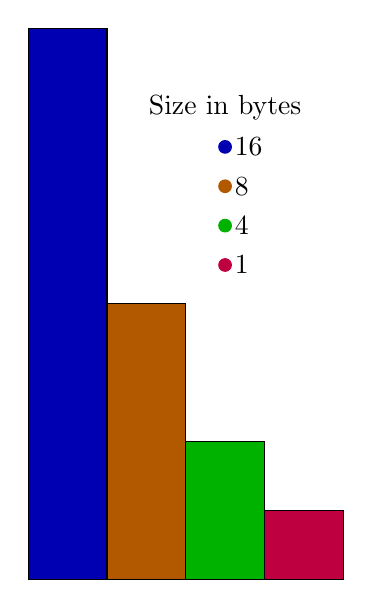
\begin{tikzpicture}[scale=1.0]
\node[anchor=south, draw,node distance=0cm, fill=nodecontc,shape=rectangle,minimum height=7.0cm  ,minimum width=1.0cm]
(node0) at (0cm,0.0cm) {};
\node[anchor=south,draw,node distance=0cm, fill=bothcontc,shape=rectangle,minimum height=3.5cm  ,minimum width=1.0cm]
(node1) at (1cm,0.0cm) {};
\node[anchor=south,draw,node distance=0cm, fill=arraycontc,shape=rectangle,minimum height=1.75cm  ,minimum width=1.0cm]
(node2) at (2cm,0.0cm) {};
\node[anchor=south,draw,node distance=0cm, fill=purple,shape=rectangle,minimum height=0.875cm  ,minimum width=1.0cm]
(node3) at (3cm,0.0cm) {};

\node[] at (2cm,6.0cm) {\color{black} Size in bytes};
\filldraw[nodecontc] (2cm,5.5cm) circle (0.08cm) node[right] {\color{black} 16};
\filldraw[bothcontc] (2cm,5.0cm) circle (0.08cm) node[right] {\color{black}8};
\filldraw[arraycontc] (2cm,4.5cm) circle (0.08cm) node[right] {\color{black}4};
\filldraw[purple] (2cm,4.0cm) circle (0.08cm) node[right] {\color{black}1};

\end{tikzpicture}

\end{column}
\begin{column}{0.5\textwidth}

\begin{lstlisting}
struct node1 {     // sizeof (node2) = 4
  std::uint8_t n;  // 256 elements.
  std::uint8_t v;  // [0, 256]
};

struct node2 {     // sizeof (node2) = 4
  std::uint16_t n; // 2^16 elements.
  std::uint16_t v; // [0, 2^16]
};

struct node3 {     // sizeof (node3) = 8
  std::uint32_t n; // 2^32 elements.
  std::uint32_t v; // [0, 2^32]
};

struct node4 {     // sizeof (node4) = 16
  node* next;      // Full address space
  std::size_t v;
};

\end{lstlisting}

\end{column}
\end{columns}

\end{frame}

%____________________________________________________________
\begin{frame}{}
    \vspace{1cm}
    \begin{center}
        {\Large \bf Thank you! Questions?} 
    \end{center}
\end{frame}

\end{document}


